\chapter{Literature Review}
\label{chapterlabel2}
    \section{Estimate mobility Flows} 

     Flow generation aims to synthesise real flow patterns between different geographical locations. It involves considering the specific attributes of these locations, such as population density, Points of Interest (POIs), land use characteristics, and the distances among them. This process is executed without direct access to real-world flow data, highlighting the dependence on generative models to represent mobility patterns accurately \citep{lucaSurveyDeepLearning2021}.
    
    Moreover, Mobility data captured through electronic devices provide invaluable insights into the movements of individuals over specific time intervals\citep{lucaSurveyDeepLearning2021}. These movements are recorded as spatiotemporal trajectories or aggregated mobility flows. Spatiotemporal trajectories and spatial aggregations, such as spatial-temporal points and tessellation, are crucial in this analysis as foundational elements for analysing and modelling mobility patterns\citep{lucaSurveyDeepLearning2021, siminiDeepGravityModel2021}.
    
    The implications of flow generation extend across various sectors, including urban planning, spatial economics, sustainable community design, and epidemiological modelling. The ability to generate accurate mobility flows is critical for addressing issues related to transportation planning, reducing socioeconomic inequalities, designing resilient communities, and understanding the spread of diseases within populations\citep{lucaSurveyDeepLearning2021}. Thus, the focus on flow generation and the generation of realistic mobility trajectories holds promise for enhancing various aspects of urban planning, spatial analysis, and public health.
      
    \section{Spatial Interaction models}

    A significant moment in the research of flow estimation was in 1946 when George K. Zipf introduced a conceptual framework for estimating mobility flows\citep{siminiDeepGravityModel2021, wilkinsonSpatialInteractionModels2023}. This model illustrated a parallel with Newton's universally accepted law of gravitation. This model, known as the gravity model, assumes that the amount of travellers moving between two specific locations is directly proportional to the population size of these locations. In parallel, this flow decreases in inverse proportion to their spatial separation\citep{wilsonFamilySpatialInteraction1971b}.
        
    While the gravity model has gained considerable attention due to its notable outcomes, some limitations exist. In particular, the gravity model needs help accurately capture some patterns inherent in real-world flows\citep{wilkinsonSpatialInteractionModels2023}. Furthermore, the generative process of flows, as predicted by the gravity model, does not consider the influence of other factors, such as Points of Interest (POIs), street networks, and other contextual variables\citep{lucaSurveyDeepLearning2021}.

    Besides that, spatial interaction models have some limitations in handling extensive datasets, such as loyalty card information, where basic calibration techniques can face constraints due to computational capabilities. \citep{wilkinsonSpatialInteractionModels2023}
    
    In parallel, some alternatives, such as the production-constrained model, have emerged to improve and extend the gravity model's efficacy. The Production-Constrained Model, conceived by \cite{wilsonFamilySpatialInteraction1971b}, introduces a key adjustment to traditional modelling techniques. Instead of relying on a single constant of proportionality, denoted as K, this model substitutes it with a set of constants commonly referred to as 'balancing factors.' This innovative approach allows more integration of additional knowledge as constraints within the modelling framework.

    The production-constrained or retail model considers critical input data, specifically the population distribution and corresponding purchasing power, to arrive at meaningful insights\citep{wilsonFamilySpatialInteraction1971b}. Related to transport, the production-attraction-constrained model serves as a valuable tool. It operates assuming that 'trip ends,' which denote the predetermined number of origins and destinations within each zone for a given type of trip, are available as input data. The primary aim of this model is to estimate the attractiveness factor based on this crucial information. To illustrate, constructing a model to analyse commuting patterns corresponds to the number of residents working in a region and the number of jobs\citep{wilsonFamilySpatialInteraction1971b}. This innovative approach provides a more comprehensive understanding of the dynamics involved in various scenarios and underscores the versatility of the production-constrained model in diverse analytical contexts.



    \section{Deep Learning for mobility flows}

    The application of neural network methodology in spatial interaction modelling marked a significant advancement in data science methodologies. A new approach from traditional models could provide more accurate predictions. \citep{wilkinsonSpatialInteractionModels2023}
        
    Comparative studies between neural network models and established frameworks revealed promising insights. These investigations indicated that neural networks could surpass the predictive accuracy of the Wilsonian model (Fischer \& Gopal, 1994; Black, 1995). However, it is crucial to note that these neural network models were frequently contrasted against unconstrained Ordinary Least Squares (OLS) calibrated models, raising queries about the true advantages of neural networks in spatial interaction modelling (Mozolin et al., 2000). \citep{wilkinsonSpatialInteractionModels2023}
        
    Incorporating neural networks presents specific challenges. The key requirement is the development of loss functions that are unambiguous, relevant, and clear. These functions play a pivotal role in estimating the total income of retail stores. The complexities of this implementation are highlighted in the iterative calibration phase, where the reliance on metrics such as average trip distance is emphasised. Thus, it is crucial to carefully consider and calibrate neural networks to ensure accurate revenue estimation in the grocery retail sector. \citep{wilkinsonSpatialInteractionModels2023}
        
    The early applications of neural networks in spatial interaction modelling demonstrated their potential to enhance predictive accuracy in commodity flows, trade, and migration domains. However, a comprehensive understanding of their advantages over traditional models requires more nuanced comparative assessments\citep{wilkinsonSpatialInteractionModels2023}.

    Deep Learning models offer the advantage of a high perfomance in capturing complex mobility patterns, a valuable method for flow generation. However, it is important to note their effectiveness on the data they are trained on, raising questions about their applicability across different geographical contexts. \citep{wilkinsonSpatialInteractionModels2023}

    \cite{lucaSurveyDeepLearning2021} study aims to investigate the use of deep learning techniques in mobility-related tasks. The research focuses on estimating mobility flows, particularly on generating realistic trajectories that replicate actual movement patterns. The study aims to enhance our understanding of complex mobility networks and their applications in various domains by utilising deep learning.

    Besides that, an inherent characteristic of Deep Learning models is their opacity, often called "black boxes". As stated by \cite{lucaSurveyDeepLearning2021}, This opacity can make interpreting the underlying logic behind generating trajectories or predicting locations and flows challenging. Nevertheless, interpretability is essential to comprehend mobility patterns and uncover potential biases in the model's decision-making process.
        
    According to \cite{lucaSurveyDeepLearning2021}, while Deep Learning models offer promise, they also introduce privacy concerns during the training and prediction phases. For instance, a critical issue in trajectory generation lies in assessing the risk of re-identifying real individuals from synthetic trajectory data. This concern becomes even more pronounced when data availability for model training is limited.
        
    The evaluation of flow generators typically relies on commuting data obtained from official statistical institutes' censuses. The assessment of flow generation commonly revolves around calculating the Common Part Of Commuters (CPC) between real and generated flows. Additionally, widely used metrics like Mean Absolute Error (MAE), Root Mean Square Error (RMSE), and Mean Absolute Percentage Error (MAPE) are also employed for this purpose.
        
    To summarise, integrating Deep Learning into generative tasks related to mobility patterns is a relatively recent development poised to gain prominence in the near future. While these models hold the potential to unravel complex mobility dynamics, their reliance on training data, lack of transparency, privacy considerations, and evaluation metrics emphasise the multifaceted nature of their application in this domain.   

    \begin{figure}[H]
        \centering
        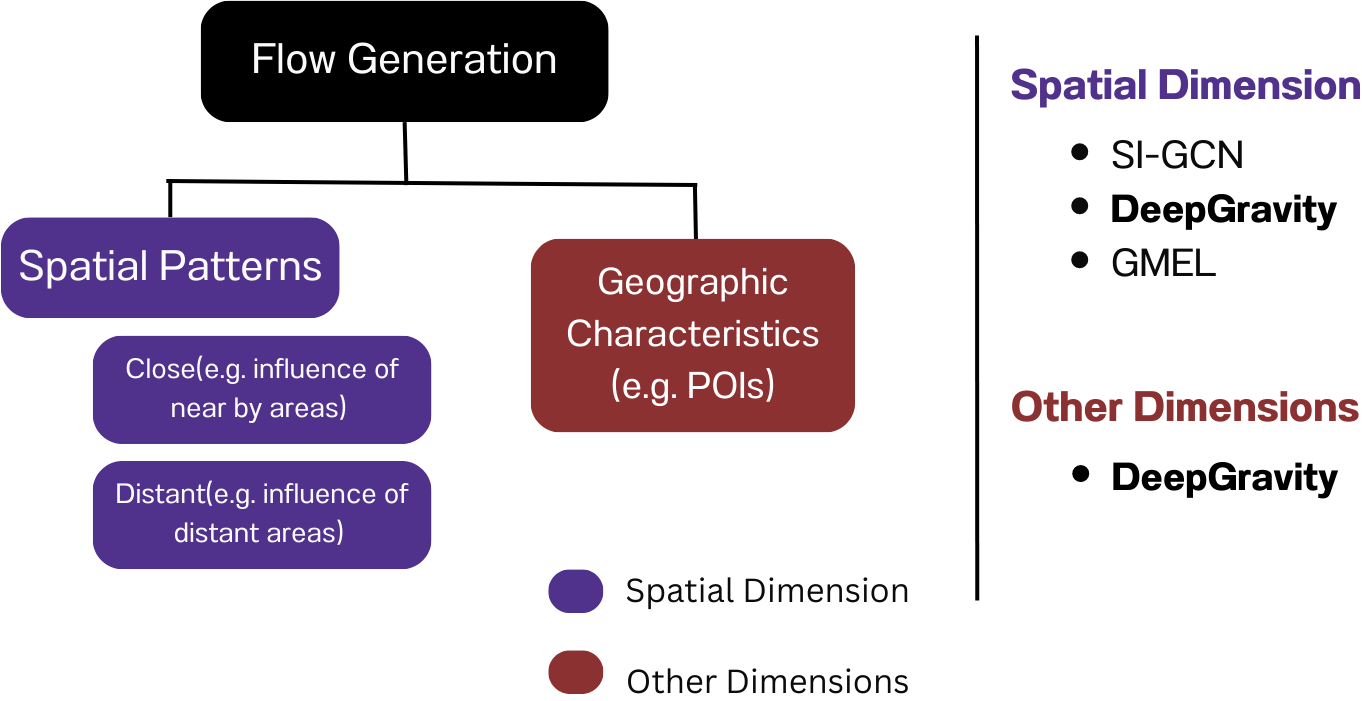
\includegraphics[width=12cm]{Images/deepgravity_fig.png}
        \caption{Deep Learning for Mobility Flows. Adapted from: \cite{lucaSurveyDeepLearning2021}}
        \label{fig: DG evaluation}
    \end{figure}

        
    \section{Deep Gravity Model}

    Deep learning methodologies have marked a significant landmark in mobility studies, particularly in analysing and predicting mobility flows. Some studies have presented the potential of deep learning techniques to encapsulate complex relationships embedded within mobility data while also drawing attention to the challenges inherent in the inherent opacity of these models, such as privacy concerns and the salient role of geographic features in enhancing the fidelity of flow predictions.

    Luca et al.'s study underscores the unique capacity of deep learning models to navigate intricate and non-linear associations within the data. This feature enables the seamless assimilation of supplementary data about specific locations, such as population density and Points of Interest (POIs). This feat eludes conventional spatial interaction models. This novel approach drives the understanding of mobility patterns beyond the linear models, providing a more holistic comprehension\citep{lucaSurveyDeepLearning2021}.

    \cite{lucaSurveyDeepLearning2021}'s work lies in the innovative concept of the Common Part of Commuters (CPC), an instrumental metric that assesses flow generator performance. This metric involves a comparative analysis of the model-generated flows against real-world data, thereby quantifying the accuracy of predictions. In addition to CPC, the study underscores the significance of employing a diverse array of evaluation metrics, including Mean Absolute Error (MAE), Root Mean Squared Error (RMSE), and Mean Absolute Percentage Error (MAPE), to offer a comprehensive understanding of model efficacy (Luca et al., 2021). 

    Beyond the technical aspects, the research presents the challenges tied to the inherent opacity of deep learning models, spotlighting the critical need to address privacy concerns, especially in scenarios involving trajectory generation where limited data availability poses a formidable obstacle (Luca et al., 2021).

    Simini et al.'s work, adds a new dimension to the discourse by delving into flow prediction and generation. A key aspect of their approach is the strategic application of geographic features extracted from OpenStreetMap to improve the accuracy of mobility flow predictions. This strategic incorporation of geographical attributes forms the bedrock upon which the Deep Gravity model, a deep neural network, is trained.
 
    The acknowledgement of the opacity challenge intrinsic to deep learning models is worth highlighting, which they address by supporting the input of explainable AI techniques to enhance the interpretability and transparency of the model's decision-making process (Simini et al., 2021).

    Regarding model performance, Simini et al.'s research shed light on the superior efficacy of the Deep Gravity model vis-à-vis conventional shallow neural networks and established gravity models. This contrast in performance underscores the intrinsic potency of deep learning in uncovering nuanced relationships within geographical attributes, ultimately yielding more precise flow predictions (Simini et al., 2021). .

    The study also highlights the pivotal role of the intricate interplay of diverse geographic features, particularly in densely populated regions. This intricate dance of geographic attributes significantly enhances the model's predictive capabilities, especially in scenarios where traditional models fall short (Simini et al., 2021).

    In summary, the combined endeavours of Luca et al. (2021) and Simini et al. (2021) offer an insightful glimpse into the potential of deep learning models to decode and simulate the complex tapestry of mobility flows. These studies collectively illuminate the capacity of these models to untangle intricate relationships embedded within mobility data and underscore the significance of embedding geographic features to elevate the precision of flow predictions.

    While these studies grapple with the challenges of model opacity and privacy concerns, they collectively herald the transformative potential of deep learning in enhancing our understanding of mobility patterns. By extrapolating from these findings, the Deep Gravity model emerges as a promising contender for replication across a diverse spectrum of contexts, effectively transcending the constraints of census data that formed the foundation of the original studies. 

    This extension holds the promise of extracting invaluable insights from high-accuracy datasets, as exemplified in the bustling urban milieu of London, potentially revolutionising the landscape of urban planning and decision-making.



    \section{Conclusion}

    In this literature review, we have explored the importance of estimating mobility flows and the relevance of spatial interaction models in this context, focusing on recent developments in deep learning models. Flow estimation, crucial for understanding urban mobility, involves synthesising patterns of movement between different geographical locations, considering factors such as population density, Points of Interest (POIs), land use, and distances. These flow patterns play a pivotal role in various domains, including urban planning, spatial economics, community design, and epidemiological modelling, addressing challenges related to transportation planning, socioeconomic disparities, community resilience, and disease spread.

    Spatial interaction models offer valuable insights into flow estimation but have limitations in capturing complex real-world patterns and considering contextual factors like POIs and street networks. On the other hand, Deep learning models have brought significant advancements in mobility flow estimation, surpassing traditional models' predictive accuracy. These models excel in capturing complex relationships within mobility data, albeit with concerns about their opacity and privacy implications.

    The Deep Gravity model, combining geographic features from OpenStreetMap with deep neural networks, demonstrates superior performance in flow prediction compared to conventional models, further emphasizing the potential of deep learning in unravelling nuanced relationships within geographical attributes. The studies collectively suggest that these models can improve our understanding of mobility patterns, especially when applied to high-accuracy datasets in urban planning and decision-making contexts.